% This is a Basic Assignment Paper but with like Code and stuff allowed in it. 

\documentclass[11pt]{article}

% Preamble

\usepackage[margin=1in]{geometry}
\usepackage{amsfonts, amsmath, amssymb}
\usepackage{fancyhdr, float, graphicx}
\usepackage[utf8]{inputenc} % Required for inputting international characters
\usepackage[T1]{fontenc} % Output font encoding for international characters
\usepackage{fouriernc} % Use the New Century Schoolbook font
\usepackage[nottoc, notlot, notlof]{tocbibind}
\usepackage{listings}
\usepackage{xcolor}

\definecolor{codegreen}{rgb}{0,0.6,0}
\definecolor{codegray}{rgb}{0.5,0.5,0.5}
\definecolor{codepurple}{rgb}{0.58,0,0.82}
\definecolor{backcolour}{rgb}{0.95,0.95,0.92}

\lstdefinestyle{mystyle}{
    backgroundcolor=\color{backcolour},   
    commentstyle=\color{codegreen},
    keywordstyle=\color{magenta},
    numberstyle=\tiny\color{codegray},
    stringstyle=\color{codepurple},
    basicstyle=\ttfamily\footnotesize,
    breakatwhitespace=false,         
    breaklines=true,                 
    captionpos=b,                    
    keepspaces=true,                 
    numbers=left,                    
    numbersep=5pt,                  
    showspaces=false,                
    showstringspaces=false,
    showtabs=false,                  
    tabsize=2
}

\lstset{style=mystyle}

% Header and Footer
\pagestyle{fancy}
\fancyhead{}
\fancyfoot{}
\fancyhead[L]{\textit{\Large{OOPJC Assignment 2}}}
%\fancyhead[R]{\textit{something}}
\fancyfoot[C]{\thepage}
\renewcommand{\footrulewidth}{1pt}



% Other Doc Editing
% \parindent 0ex
%\renewcommand{\baselinestretch}{1.5}

\begin{document}

\begin{titlepage}
	\centering

	%---------------------------NAMES-------------------------------

	\huge\textsc{
		MIT World Peace University
	}\\

	\vspace{0.75\baselineskip} % space after Uni Name

	\LARGE{
		Object Oriented Programming with Java and C++\\
		Second Year B. Tech, Semester 1
	}

	\vfill % space after Sub Name

	%--------------------------TITLE-------------------------------

	\rule{\textwidth}{1.6pt}\vspace*{-\baselineskip}\vspace*{2pt}
	\rule{\textwidth}{0.6pt}
	\vspace{0.75\baselineskip} % Whitespace above the title



	\huge{\textsc{
			Implementation of Inheritance using C++ and Java
		}} \\



	\vspace{0.5\baselineskip} % Whitespace below the title
	\rule{\textwidth}{0.6pt}\vspace*{-\baselineskip}\vspace*{2.8pt}
	\rule{\textwidth}{1.6pt}

	\vspace{1\baselineskip} % Whitespace after the title block

	%--------------------------SUBTITLE --------------------------	

	\LARGE\textsc{
		Practical Report
	} % Subtitle or further description
	\vfill

	%--------------------------AUTHOR-------------------------------

	Prepared By
	\vspace{0.5\baselineskip} % Whitespace before the editors

	\Large{
		Krishnaraj Thadesar \\
		Cyber Security and Forensics\\
		Batch A1, PA 20
	}


	\vspace{0.5\baselineskip} % Whitespace below the editor list
	\today

\end{titlepage}


\tableofcontents
\thispagestyle{empty}
\clearpage


\setcounter{page}{1}

\section{Aim and Objectives}
\subsection*{Aim}
To Implement inheritance using C++ and Java (with interfaces).
\subsection*{Objectives}
\begin{enumerate}
	\item To understand the inheritance or is-A relationship concept.
	\item To understand code reusability.
	\item To learn implementation of interfaces in java.
\end{enumerate}
\section{Problem Statements}
\subsection{Problem 1 in C++}

Design and develop inheritance for a given case study, identify objects and relationships
and implement inheritance wherever applicable using C++.\\
Employee class has Empname, Empid, Address, Mailid, and Mobileno as data
members.
Add the Following Classes
\begin{itemize}
	\item Programmer
	\item Team Leader
	\item Assistant Project Manager
	\item Project Manager from Employee Class
\end{itemize}
\noindent
Add Basic Pay as the member of all the inherited classes with 97 \% of the Basic Pay as DA, 10 \% of Basic Pay as HRA, 12 \% of  Basic Pay as PF, 0.1 \% of Basic Pay for staff club fund.

Generate Pay slips for the Employees with their gross and net salaries.

\subsection{Problem 2 in Java}
Write a Java Program for demonstrating Inheritance in Java.
Write a program in Java showing hierarchical inheritance with base class as Employee and
derived classes as FullTimeEmployee and InternEmployee with methods DisplaySalary in
base class and CalculateSalary in derived classes.
Calculate salary method will calculate as per increment given to fulltime and intern
Employees. Fulltime employee- 50\% hike, Intern employee-25\% hike. Display salary
before and after hike.
\subsection{Probelm 3 in Java}
Write a java program to create two interfaces Motorbike and Cycle.
\begin{itemize}
	\item Motorbike interface consists of the attribute speed.
	\item The method is totalDistance().
	\item Cycle interface consists of the attributes distance and the method speed().
	\item These interfaces are implemented by the class TwoWheeler.
	\item Calculate total distance travelled and Average Speed maintained by Two Wheeler.
\end{itemize}

\section{Theory}

\subsection{Concept of Inheritance and its types}
\textbf{Inheritance} is a process in which one object acquires all the properties and behaviors of its parent object automatically. In such way, you can \textit{reuse, extend, or modify} the attributes and behaviors which are defined in other class.

In C++, the class which inherits the members of another class is called derived class and the class whose members are inherited is called base class. The derived class is the specialized class for the base class. Most ideas of inheritance are directly applicable in Java as well.


\subsubsection{Advantages}
\begin{enumerate}
	\item Minimizing duplicate code: Key benefits of Inheritance include minimizing the identical code as it allows sharing of the common code among other subclasses.

	\item Flexibility: Inheritance makes the code flexible to change, as you will adjust only in one place, and the rest of the code will work smoothly.

	\item Overriding: With the help of Inheritance, you can override the methods of the base class.

	\item Data Hiding: The base class in Inheritance decides which data to be kept private, such that the derived class will not be able to alter it.
\end{enumerate}

\subsubsection{Types of Inheritance}

\begin{enumerate}
	\item Single inheritance :
	      It is defined as the inheritance in which a derived class is inherited from the only one base class.
	\item Multiple inheritance : It is the process of deriving a new class that inherits the attributes from two or more classes.
	\item Hierarchical inheritance : When one class inherits another class which is further inherited by another class, it is known as multi level inheritance in C++. Inheritance is transitive so the last derived class acquires all the members of all its base classes.
	\item Multilevel inheritance: It is a process of deriving a class from another derived class.
	\item Hybrid inheritance : Any legal combination of any of the above inheritance techniques would be known as hybrid inheritance.
\end{enumerate}

\textbf{Let us Look an Examples of these.}
\begin{lstlisting}[language = C++]
	class A
	{
		// Base Class
	};

	class D
	{
		// Base Class 2
	}
	class B : public A
	{
		// Single Inheritance
	}
	class C : public B
	{
		// Multi Level Inheritance
	}
	class E : public A, public D
	{
		// Multiple Inheritance
	}
	class F : public E, private D
	{
		// hierarchical inheritance
	}
\end{lstlisting}

\subsubsection{Base class and Derived Class Constructors}
Whenever we create an object of a class, the default constructor of that class is invoked automatically to initialize the members of the class. \\

If we inherit a class from another class and create an object of the derived class, it is clear that the default constructor of the derived class will be invoked but before that the default constructor of all of the base classes will be invoke, i.e the order of invocation is that the base class's default constructor will be invoked first and then the derived class's default constructor will be invoked.\\

When a class is inherited from other, The data members and member functions of base class comes automatically in derived class based on the access specifier but the definition of these members exists in base class only. So when we create an object of derived class, all of the members of derived class must be initialized but the inherited members in derived class can only be initialized by the base class's constructor as the definition of these members exists in base class only. \\

This is why the constructor of base class is called first to initialize all the inherited members.

\subsubsection*{Let us see an Example}

\begin{lstlisting}[language = C++]
 
// base class
class Parent
{
    public:
     
    // base class constructor
    Parent()
    {
        cout << "Inside base class" << endl;
    }
};
 
// sub class
class Child : public Parent
{
    public:
     
    //sub class constructor
    Child()
    {
        cout << "Inside sub class" << endl;
    }
};
 
// main function
int main() {
      
    // creating object of sub class
    Child obj;

    return 0;
}
	
\end{lstlisting}
\textbf{Output would be}
\begin{verbatim}
	Inside base class
	Inside sub class
\end{verbatim}

\section{Platform}
\textbf{Operating System}: Arch Linux x86-64\\
\textbf{IDEs or Text Editors Used}: Visual Studio Code\\
\textbf{Compilers} : g++ and gcc on linux for C++, and javac, with JDK 18.0.2 for Java\\

\section{Input}

\subsection*{For C++}
\begin{enumerate}
	\item Number of Each Type of Employee
	\item Name, Age, Address City, and Salary of Each Employee
\end{enumerate}

\subsection*{For Java}
\begin{enumerate}
	\item The Information and Salary about the Full Time Employee
	\item The Information and Salary of the Intern Employee
	\item Speed, Time and Distance
\end{enumerate}

\section{Output}
\subsection*{For C++}
\begin{enumerate}
	\item General Information about Each Employee
	\item The Gross Salary of Each Employee
	\item The Net Salary of Each Employee
\end{enumerate}

\subsection*{For Java}
\begin{enumerate}
	\item The General information about the Full time and the Intern Employee
	\item The Hiked salaries of both the Intern Employee, and the Full Time Employee.
	\item Speed and Distance.
\end{enumerate}


\section{Code}

\subsection{C++ Implementation for Problem 1}

\lstinputlisting[language=c++, caption=Main.Cpp]{../Programs/cpp_implementations/Assignment_2.cpp}

\subsubsection{C++ Input and Output}
\begin{lstlisting}[language=bash, caption=C++ Output]

Welcome to Employee Payroll Management System

Whose Details do you wanna enter?
1. Programmer
2. Team Leader
3. Assistant Project Manager
4. Project Manager
5. Quit
1
How many Programmers are we talking? 1
The Default Constructor was called
Enter the Information about the Programmer
Enter the Employee ID:
1001
Enter the Employee Name:
Tony
Enter the Employee Age:
45
Enter the Employee Address City:
Berlin
Enter the basic Salary of the Programmer :
450000

Here is their Information and their Pay Slips


Programmer
Info and Pay Slip of Programmer 1
Employee ssn is:1001
Employee ID is : 1001
Employee Name: Tony
Employee Age: 45
Employee Address City: Berlin
The Gross Salary is: 2.2365e+06
The Net Salary is: 1.90102e+06

The Destructor was called


Whose Details do you wanna enter?
1. Programmer
2. Team Leader
3. Assistant Project Manager
4. Project Manager
5. Quit
2
How many Team Leaders are we talking? 1
The Default Constructor was called
Enter the Information about the Team Leader 1
Enter the Employee ID:
1002
Enter the Employee Name:
Steve
Enter the Employee Age:
80
Enter the Employee Address City:
Queens
Enter the basic Salary of the Team Leader :
70000
Here is their Information and their Pay Slips


Info and Pay Slip of Team Leader 1
Employee ssn is:1002
Employee ID is : 1002
Employee Name: Steve
Employee Age: 80
Employee Address City: Queens
The Gross Salary is: 347900
The Net Salary is: 295715



The Destructor was called


Whose Details do you wanna enter?
1. Programmer
2. Team Leader
3. Assistant Project Manager
4. Project Manager
5. Quit
3
How many Assistant Project Managers are we talking? 1
The Default Constructor was called
Enter the Information about the Assitant Project Manager 1
Enter the Employee ID:
1003
Enter the Employee Name:
Caulson
Enter the Employee Age:
60
Enter the Employee Address City:
Delhi
Enter the basic Salary of the Assistant Project Manager :
60000
Here is their Information and their Pay Slips


Info and Pay Slip of Assitant Project Manager 1
Employee ssn is:1003
Employee ID is : 1003
Employee Name: Caulson
Employee Age: 60
Employee Address City: Delhi
The Gross Salary is: 298200
The Net Salary is: 253470



The Destructor was called


Whose Details do you wanna enter?
1. Programmer
2. Team Leader
3. Assistant Project Manager
4. Project Manager
5. Quit
4
How many Project Managers are we talking? 1
The Default Constructor was called
Enter the Information about the Project Manager 1
Enter the Employee ID:
1005
Enter the Employee Name:
Fury
Enter the Employee Age:
56
Enter the Employee Address City:
Pune
Enter the basic Salary of the Project Manager :
600000
Here is their Information and their Pay Slips


Info and Pay Slip of Project Manager 1
Employee ssn is:1004
Employee ID is : 1005
Employee Name: Fury
Employee Age: 56
Employee Address City: Pune
The Gross Salary is: 2.982e+06
The Net Salary is: 2.5347e+06

The Destructor was called


Whose Details do you wanna enter?
1. Programmer
2. Team Leader
3. Assistant Project Manager
4. Project Manager
5. Quit
5
\end{lstlisting}

\subsection{Java Implementation of Problem 2}

\lstinputlisting[language=java, caption=Employee.java]{../Programs/java_implementations/assignment_2/Employee.java}
\lstinputlisting[language=java, caption=Intern Employee.java]{../Programs/java_implementations/assignment_2/InternEmployee.java}
\lstinputlisting[language=java, caption=Full Time Employee.java]{../Programs/java_implementations/assignment_2/FullTimeEmployee.java}
\lstinputlisting[language=java, caption=Main.java]{../Programs/java_implementations/assignment_2/Main.java}

\subsubsection{Java Output for Problem 2}
\begin{lstlisting}[caption=Java Output for Problem 2]
Welcome to Salary Hiking Program
Enter the Details about the Full Time Employee:

Enter the Employee Name
Tony
Enter The Employee ID
1001
Enter The Employee Salary
100000
The Employee Name is: Tony
The Employee ID is: 1001
The Salary Before the Hike for this Full time Employee is: 100000.0
The Salary after the Hike for this Full time Employee is : 200000.0
Enter the Details about the Intern Employee:

Enter the Employee Name
Steve
Enter The Employee ID
1002
Enter The Employee Salary
50000
The Employee Name is: Steve
The Employee ID is: 1002
The Salary Before the Hike for this Intern Employee is: 50000.0
The Salary after the Hike for this Intern Employee is : 100000.0
\end{lstlisting}

\subsection{Java Implementation of Problem 3 using Interfaces}

\lstinputlisting[language=java, caption=Two Wheeler.java]{../Programs/java_implementations/assignment_2b/TwoWheeler.java}
\lstinputlisting[language=java, caption=MotorCycle.java]{../Programs/java_implementations/assignment_2b/MotorCycle.java}
\lstinputlisting[language=java, caption=Cycle.java]{../Programs/java_implementations/assignment_2b/Cycle.java}
\lstinputlisting[language=java, caption=Main.java]{../Programs/java_implementations/assignment_2b/Main.java}

\subsubsection{Java Output}
\begin{lstlisting}[caption=Java Output for Program 3]
Calculating Speed:
Enter the Distance Travelled by Your 2 Wheeler:
50
Enter the Time you Travelled on Your 2 Wheeler:
2
The Speed is:
25
Calculating Total Distance:
Enter the Speed of Your 2 Wheeler:
25
Enter the Time you Travelled on Your 2 Wheeler:
2
The Total Distance is:
50
\end{lstlisting}

\pagebreak

\section{Conclusion}
Thus, learned to use reusability by applying concept of inheritance, interfaces and
implemented solution of the given problem statement using C++ and Java.

\section{FAQs}

\begin{enumerate}
	\item \textbf{Discuss ambiguity arises in multipath inheritance and how it is to be avoided in C++?}\\
	      In \textit{multiple} inheritances, when one class is derived from two or more base classes then there may be a possibility that the base classes have functions with the same name, and the derived class may not have functions with that name as those of its base classes. \\
	      \\
	      If the derived class object needs to access one of the similarly named member functions of the base classes then it results in ambiguity because the compiler gets confused about which base's class member function should be called.

	      To solve this ambiguity scope resolution operator is used denoted by ' :: '

	      \textbf{The Syntax to use it is: }
	      \begin{lstlisting}[language=C++]
		ObjectName.ClassName::FunctionName();
	\end{lstlisting}

	      \textbf{An Example: }
	      \begin{lstlisting}[language=C++]
// C++ program to resolve inheritance
// ambiguity
 
#include<iostream>
using namespace std;
 
// Base class A
 
class A {
    public:
 
    void func() {
        cout << " I am in class A" << endl;
    }
};
 
// Base class B
 
class B {
    public:
 
    void func() {
        cout << " I am in class B" << endl;
    }
};
 
// Derived class C
class C: public A, public B {
 
 
};
 
// Driver Code
 
int main() {
 
    // Created an object of class C
    C obj;
 
    // Calling function func() in class A
    obj.A::func();
 
    // Calling function func() in class B
    obj.B::func();
 
    return 0;
}
		
	\end{lstlisting}

	\item \textbf{What's the difference between public, private, and protected?} \\
	      \textit{public, private, and protected} are known as access modifiers. Like their name suggests, they modify the access given to objects and subclasses.
	      \begin{enumerate}
		      \item If you do class child : \textbf{private} parent; then every private data member becomes inaccessible, coz anyway thats what should happen, then the protected data members become private, and public data members also become private.
		      \item If you do class child : \textbf{protected} parent; then its the same thing, except you still cant access private variables, but protected and public data members become protected
		      \item Same with class child : \textbf{public} parent; everything remains unchanged. The objects will behave in accordance with the usual laws of objects.
	      \end{enumerate}

	\item \textbf{Why can't derived class access private things from base class?}:\\
	      The \textbf{private} access modifier, when used in any class, by its definition restricts sub classes and its objects to access variables declared in its scope. As a result, derived classes can not access the private variables defined in the base class.
	      \begin{lstlisting}[language=C++]
		class A
		{
			private: 
				int a;
		};
		class B: public A
		{
			
		}obj;
		int main()
		{
			A.a // not accessible
		}
	\end{lstlisting}
	      \pagebreak
	\item \textbf{Explain use of 'super' keyword with suitable example}\\
	      The \textit{super} keyword in Java refers to the parent class's variables and functions. Whenever you create the instance of subclass, an instance of parent class is created implicitly which is referred by super reference variable.

	      \begin{itemize}
		      \item super can be used to refer immediate parent class instance variable.
		      \item super can be used to invoke immediate parent class method.
		      \item super() can be used to invoke immediate parent class constructor.
	      \end{itemize}
	\item \textbf{Why to use concept of interface in Java}\\

	      An \textbf{Interface} in Java programming language is defined as an abstract type used to specify the behavior of a class. An interface in Java is a blueprint of a class. A Java interface contains static constants and abstract methods.\\
	      The interface in Java is a mechanism to achieve abstraction. There can be only abstract methods in the Java interface, not the method body. It is used to achieve abstraction and multiple inheritance in Java. In other words, you can say that interfaces can have abstract methods and variables. It cannot have a method body. Java Interface also represents the IS-A relationship.\\

	      Like a class, an interface can have methods and variables, but the methods declared in an interface are by default abstract (only method signature, no body).

	      \begin{itemize}
		      \item \textbf{Provides Communication} - One of the uses of the interface is to provide communication. Through interface you can specify how you want the methods and fields of a particular type.
		      \item \textbf{Multiple Inheritance}  - Java doesn't support multiple inheritance, using interfaces you can achieve multiple inheritance.
		      \item \textbf{Abstraction}- Abstraction is a process of hiding the implementation details from the user, only the functionality will be provided to the user. In other words, the user will have the information on what the object does instead of how it does it.\\
		            Since all the methods of the interface are abstract and user doesn't know how a method is written except the method signature/prototype. Using interfaces, you can achieve (complete) abstraction.
		      \item \textbf{Loose Coupling} :  Coupling refers to the dependency of one object type on another, if two objects are completely independent of each other and the changes done in one doesn't affect the other both are said to be loosely coupled.
		            You can achieve loose coupling in Java using interfaces

	      \end{itemize}
	\item \textbf{Write Couple of Examples or Applications suitable to Demonstrate use of Inheritances.}\\
	
	Inheritance is a core part of Object Oriented Programming. In every Object oriented language, it is heavily used, and these languages are heavily used in almost all fields involving programming, which makes the uses of inheritance vast and versatile. So some of them are listed below. 
	\begin{enumerate}
		\item In Application Development: Every GUI that we see on screens, is often built on simple base classes like buttons, sliders, labels, titlebars etc. The Programmer often just inherits it, and overrides certain methods to his or her liking. 
		\item Games are built in many different ways, but as the scale of games increase it becomes pertinent to use simple base classes like trees, enemies, players, friends, coins, As there might be several of the same kind of enemies, and several sorts of trees in the game environment, which will all inherit the base class and override or create certain new methods. 
		\item In Data Science, Many algorithms are their own predefined classes, The programmer then tweaks certain parameters, and this helps them streamline and organize the process of applying this algorithm on hundreds of different datasets without hassle. 
	\end{enumerate}

	\begin{lstlisting}[language = Java]
		// Here is an example of Creating a GUI in Java using Swing. 

		// This is the definition of the JButton class, which is used for placing buttons on the screen. 
		public class JButton extends AbstractButton implements Accessible  


		import javax.swing.*;    
		public class ButtonExample {  
			public static void main(String[] args) {  

				JFrame f=new JFrame("Button Example");  
				JButton b=new JButton("Click Here");

				b.setBounds(50,100,95,30);  
				f.add(b);  
				f.setSize(400,400);  
				f.setLayout(null);  
				f.setVisible(true);   
			}  
		}  
		
	\end{lstlisting}
	
	\begin{figure}[H]
		\centering
		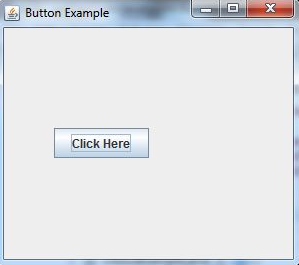
\includegraphics[scale=1]{button.png}
	\end{figure}
	

\end{enumerate}

\end{document}